\documentclass[../thesis.tex]{subfiles}
\graphicspath{{../gfx/}{gfx/}}
\begin{document}

\pagestyle{plain}

\chapter{Założenia i wymagania systemu}

Zdefiniowanie wymagań ma bardzo duże znaczenie podczas realizacji projektu informatycznego. Właściwe sformułowanie wymagań uszczegóławia wizję systemu oraz jest źródłem wiedzy o pożądanych możliwościach i cechach rozwiązania. Dodatkowo, prawidłowa identyfikacja wymagań nakreśla cel projektu i, co za tym idzie, pozwala uniknąć potrzeby wprowadzania kosztownych poprawek.

Wymagania dzielimy na funkcjonalne, jakościowe (niefunkcjonalne) oraz wymagania ograniczeń. Do pierwszej grupy zaliczamy wymagania opisujące możliwości, jakie projektowany system daje użytkownikom. Przykładem wymagania funkcjonalnego może być klasyfikowanie danych przy użyciu algorytmu drzew decyzyjnych. Wymagania jakościowe skupiają się na ilościowych regułach oceniania systemu, np. czy baza danych potrafi odzyskać utracone dane w mniej niż jedną sekundę. Ostatnia kategoria wymagań precyzuje granice rozwiązania. 

\section{Wymagania funkcjonalne}

Zgodnie z tym, co opisane jest w rozdziale poświęconym celowi pracy, przygotowywany przeze mnie system służy porównywaniu jakości klasyfikacji wielu zbiorów algorytmów. Użytkownik systemu powinien być w stanie wprowadzić informacje o rodzinach algorytmów, które chce porównać pod kątem pewnej miary jakości klasyfikacji. Użytkownik powinien również dostarczyć dane medyczne zapisane w pewnym ustalonym formacie. W efekcie tego system powinien zwrócić dane o cechach szczególnych wprowadzonych rodzin algorytmów (np. wartość średnia oceny). Dodatkowo system powinien uszeregować rodziny algorytmów pod kątem wybranej miary jakości, dając w ten sposób pogląd na wzajemną skuteczność rodzin algorytmów. Informacje o wzajemnej skuteczności rodzin mogą okazać się pomocne przy późniejszym decydowaniu, na której z rodzin należy skoncentrować dalsze badania.

Takie spojrzenie na podstawowe wymagania pozwala wyróżnić trzy podstawowe zestawy funkcjonalności: wprowadzanie danych wejściowych, wykonywanie obliczeń i prezentację wyników.

\subsection{Wprowadzanie danych wejściowych}
\label{req:input}

Jednym z podstawowych zadań systemu jest wstępne przetwarzanie danych, klasyfikacja oraz obliczenie miary jakości klasyfikacji. Taki ciąg obliczeń w reszcie pracy dla uproszczenia nazywać będę \emph{algorytmem}. Użytkownik, rozpoczynając obliczenia, powinien wprowadzić informacje o rodzinie algorytmów, dla których wyniki oceny chce uzyskać. Każdy algorytm będzie wykonywał pewne operacje na dostarczonym zbiorze danych. Aby ustalić przebieg działania pojedynczego algorytmu należy najpierw przyjrzeć się posiadanym danym biomedycznym.

\subsubsection{Opis danych wejściowych}

Dostępny zbiór danych zawiera ok. 1000 obserwacji. Każda z nich to zestaw prawdziwych, anonimowych danych otrzymanych w wyniku przebadania pacjentek pod kątem zachorowalności na raka piersi. Każda obserwacja w próbie zawiera sześć atrybutów ciągłych oraz jedną dyskretną kategorię chorobową (choruje/nie choruje). 

Pierwszym atrybutem w każdej obserwacji jest wiek pacjentki. Kolejne pięć to poziomy ekspresji:
\begin{enumerate}
  \item Swoistego antygenu sterczowego (PSA, z ang. \emph{prostate-specific antigen})
  \item Czynnika martwicy guza alfa (TNFA, z ang. \emph{tumor necrosis factor-alpha})
  \item Interleukiny 6
  \item Interleukiny 8
  \item Czynnika wzrostu śródbłonka naczyniowego (VEGF, z ang. \emph{vascular endothelial growth factor})
\end{enumerate}
Zbiór danych zawiera zbliżoną liczbę obserwacji ze stanem chorobowym oraz bez stanu chorobowego.

Dodatkowo, zestaw danych biomedycznych posiada ok. 8\% brakujących wartości różnych atrybutów (kategoria nie zawiera braków).

\begin{figure}[h]
\centering
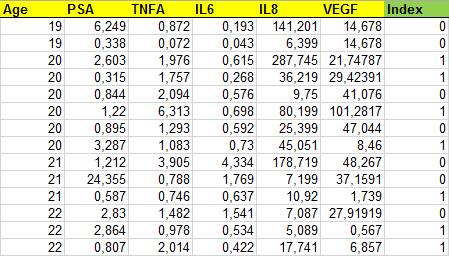
\includegraphics{data.png}
\caption{Fragment zbioru danych dotyczących zachorowalności na raka piersi u kobiet wraz z wyszczególnionymi atrybutami i kategorią (\textit{Index}).}
\label{req:data}
\end{figure}

\subsubsection{Pojedynczy algorytm}

Każdy algorytm składa się z czterech etapów wstępnego przetwarzania oraz z pojedynczego etapu końcowej klasyfikacji:
\begin{enumerate}
	\item Przetwarzanie wstępne
	\begin{enumerate}
		\item Metoda imputacji danych brakujących
		\item Wskazanie atrybutów do usunięcia
		\item Wskazanie atrybutów do przeskalowania
		\item Określenie metod grupowania i ich parametrów, wybór atrybutów do zgrupowania
	\end{enumerate}
	\item Metoda klasyfikacji wraz z parametrami
\end{enumerate}

Spośród wyżej wymienionych operacji tylko pierwsza i ostatnia powinny być zawsze określone. Wynika to z faktu, że wiele algorytmów klasyfikacji zakłada obecność wszystkich danych i nie uwzględnia sytuacji, w których pewnych wartości brakuje. Inaczej jest w przypadku pozostałych czynności. Usuwanie, skalowanie oraz grupowanie atrybutów mogą mieć zasadniczy wpływ na przebieg całego algorytmu, ale nie są konieczne. Najprostszy pojedynczy algorytm polegać będzie zatem na imputacji danych wybraną metodą oraz na późniejszej klasyfikacji danych. Najbardziej złożony algorytm zawierać będzie w sobie wszystkie wymienione etapy. 

Należy zwrócić uwagę na wymaganie dotyczące grupowania wartości w atrybutach. Aplikacja powinna pozwalać na wykorzystanie wielu różnych algorytmów łączenia jednocześnie. Dla każdego wybranego algorytmu grupowania użytkownik powinien móc wskazać zbiór atrybutów poddanych łączeniu oraz parametry algorytmu.

Fazy algorytmu związane z usuwaniem, skalowaniem i grupowaniem atrybutów wymagają wskazania zbioru atrybutów, na którym konkretna operacja ma zostać wykonana. Liczba możliwych kombinacji atrybutów zależy wykładniczo od liczby atrybutów w zbiorze. Oznacza to, że w ogólnym przypadku rodzina algorytmów nie może zawierać algorytmów ze wszystkimi możliwymi kombinacjami. Wiązałoby się to z nieakceptowalnie długim czasem obliczeń. Biorąc jednak pod uwagę, że dostępne dane zawierają tylko 6 atrybutów, można pozwolić sobie na tworzenie rodzin zawierających wszystkie kombinacje. Dalsze wymagania zakładać będą, że zbiór danych zawierać będzie nie więcej niż 10 atrybutów.

\begin{figure}[h]
\centering
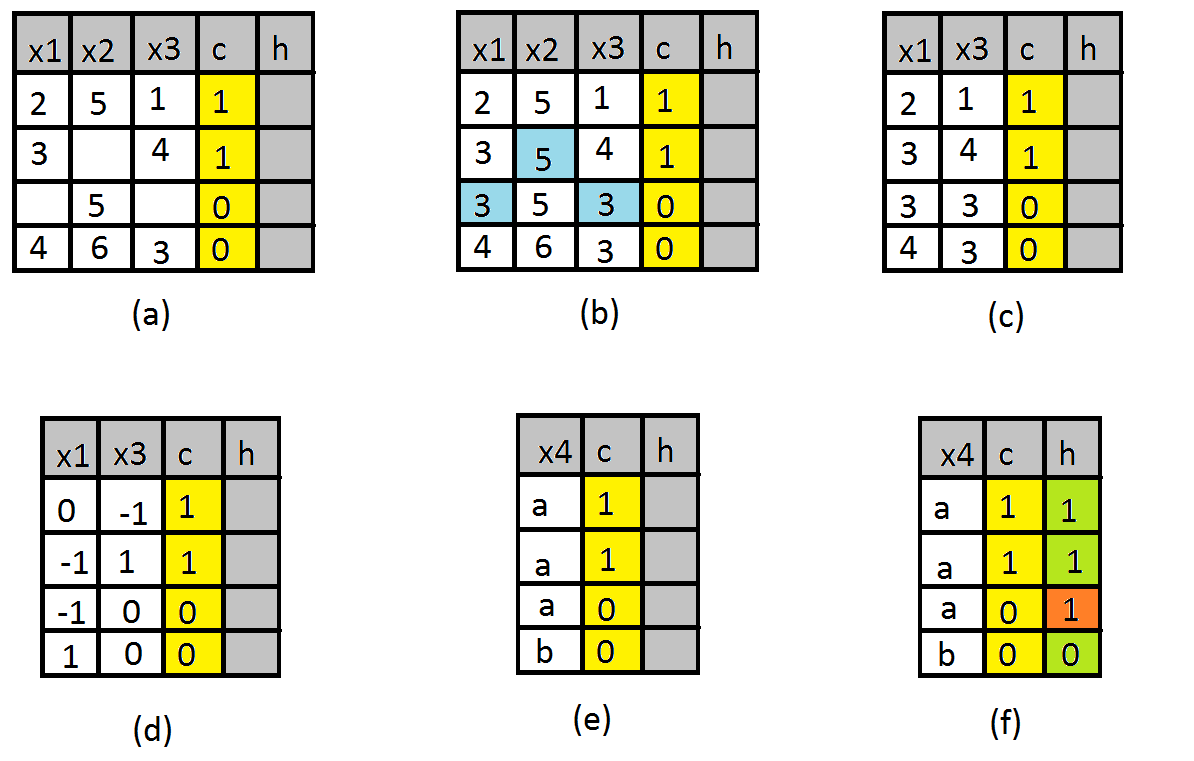
\includegraphics[width=0.8\textwidth]{algorithm.png}
\caption{Przykład działania pojedynczego algorytmu. Dane w postaci początkowej (a), po imputacji medianą (b), po usunięciu atrybutu \textit{x\textsubscript{2}} (c), po przeskalowaniu do przedziału [-1, 1] (d), po zgrupowaniu atrybutów \textit{x\textsubscript{1}} i \textit{x\textsubscript{3}} w nowy atrybut \textit{x\textsubscript{4}} (e), po predykcji wybraną metodą klasyfikacji (f).}
\label{req:algorithm}
\end{figure}

\subsubsection{Rodzina algorytmów}

System powinien obliczać jakość klasyfikacji rodziny algorytmów zdefiniowanej w pewien sposób przez użytkownika. Projektując metodę opisu rodzin algorytmów należy zachować równowagę pomiędzy jej skrótowością oraz ekspresywnością. 

Opis rozwlekły byłby kłopotliwy w użyciu, gdyż wymagałby dużego nakładu pracy, aby opisać rodzinę metod. Dokładna metoda opisu mogłaby wymagać od użytkownika bezpośredniego wprowadzania opisów kombinacji, które aplikacja miałaby obsłużyć. Jednakże przy gigantycznej liczbie wszystkich możliwych wariantów, rozwiązanie to nie znalazłoby zastosowania - opisy rodzin stałyby się po prostu za długie. 

Skrajną alternatywą mogłoby być pytanie użytkownika, czy algorytmy w rodzinie powinny uwzględniać określone operacje, np. usuwanie atrybutów lub ich grupowanie. Taki krótki, nieprecyzyjny opis nie pozwalałby na wyrażanie konkretnych rodzajów algorytmów w rodzinie.  Odpowiedzi ,,tak lub nie'' byłyby wygodne dla użytkownika, ale odbierałyby jakikolwiek wpływ na kształtowanie rodzin algorytmów.

Całkowita liczba wszystkich możliwych kombinacji metod przetwarzania wstępnego i klasyfikacji zależy wykładniczo od liczby atrybutów danych. Przykładowo, liczba możliwych kombinacji atrybutów, które aplikacja podda skalowaniu, wynosi $2^{n}$, gdzie $n$ oznacza liczbę atrybutów. Aby uniknąć długiego czasu obliczeń związanego z eksplozją wykładniczą, użytkownik powinien być w stanie określić podzbiór wszystkich kombinacji, które program ma przeanalizować. Podzbiór taki można traktować jako podprzestrzeń kombinacji parametrów wszystkich możliwych algorytmów.

Zaproponowane przeze mnie rozwiązanie stanowi kompromis pomiędzy dwoma skrajnymi metodami opisu rodzin. Polega ono na deklaratywnym opisie parametrów algorytmów należących do rodziny. 

Na samym początku użytkownik powinien wybrać metody imputacji brakujących wartości atrybutów, na przykład: $\{\emph{mediana}, \emph{wartość średnia}\}$.

W następnej kolejności użytkownik powinien określić zbiór atrybutów $R_\textrm{attr}$, spośród których aplikacja może wybrać te, które zostaną usunięte. Dodatkowo użytkownik powinien określić zbiór liczb $\textbf{R} = \{r_1, r_2, \ldots, r_n\}$, taki, że każda liczba $r_i$ oznacza liczbę atrybutów, które algorytm będzie mógł usunąć jednocześnie ze zbioru $R_\textrm{attr}$.

Analogicznie powinno przebiegać określanie szczegółów skalowania atrybutów. Użytkownik powinien wybrać zbiór atrybutów $N_\textrm{attr}$ oraz wprowadzić zbiór liczb $\textbf{N}$, którego każdy element oznaczać będzie liczbę atrybutów skalowanych jednocześnie.

Opis podprzestrzeni związanej z grupowaniem okazuje się bardziej skomplikowany. Podobnie jak poprzednio, użytkownik powinien wskazać zbiór atrybutów poddanych grupowaniu $Q_\textrm{attr}$. Następnie użytkownik powinien określić zbiór algorytmów grupowania $\textbf{Q}$, które mogą być użyte. W kolejnym kroku należy wprowadzić zbiór liczb $Q_\textrm{pass}$. Każdy element zbioru oznaczać będzie liczbę jednoczesnych przebiegów grupowania. W dalszej kolejności odbiorca określi liczbę $n_\textrm{max}$ oznaczającą maksymalną liczbę atrybutów, które mogą być łączone przez algorytmy ze zbioru $\textbf{Q}$. Na samym końcu osoba będzie musiała opisać podzbiór wszystkich kombinacji parametrów, jakie mogą przyjąć wybrane wcześniej algorytmy grupowania. Aby uprościć to zadanie, użytkownik wprowadzi tylko jedną liczbę $g$, oznaczającą \textit{granularność} podprzestrzeni parametrów. 

Wiele algorytmów często przyjmuje parametry początkowe należące do określonych dziedzin. Przykładami takich dziedzin mogą być: wartości ,,tak'' i ,,nie'', zbiór liczb rzeczywistych od $0.01$ do $100$. W ogólnym przypadku nie jest możliwe przeglądanie wszystkich kombinacji parametrów dla dowolnego algorytmu -- jest ich zbyt dużo lub ich wartości są nieprzeliczalne. Z tego powodu, w mojej pracy przeszukiwanie przestrzeni ograniczam do jej wybranych elementów. Naturalnym podejściem do tego problemu jest wybór takich wartości z każdej dziedziny, które byłby dla niej reprezentatywne. 

\emph{Granularnością} nazywam liczbę, która określa, ile równo oddalonych od siebie wartości należy wybrać z danego przedziału. Parametr ten pozwala próbkować dany przedział liczb z określoną częstością. Umożliwia to mniej lub bardziej dokładne przeglądanie parametrów liczbowych dla algorytmów grupowania i klasyfikacji. W zależności od zastosowania, różnica pomiędzy kolejnymi wartościami z przedziału może być równa na skali liniowej lub logarytmicznej.

\textit{Granularność liniową} $g_l$ dla zbioru $\{a, \ldots, b\}$ definiuję jako liczność zbioru $\textbf{L} = \{l_1, l_2, \ldots, l_n\}$ takiego, że:
\begin{eqnarray*}
&& l_1 = a \\
&& l_n = b \\
&& l_{i+1} - l_i = c
\end{eqnarray*}
gdzie $c$ jest stałą, a $i \in \{1, \ldots, n-1\}$. Intuicyjnie granularność liniowa to liczba o 1 większa od liczby podziałów zbioru na przedziały o jednakowej długości.

\textit{Granularność wykładniczą} $g_w$ dla zbioru $\{a, \ldots, b\}$ definiuję jako liczność zbioru $\textbf{W} = \{w_1, w_2, \ldots, w_n\}$ takiego, że:
\begin{eqnarray*}
&& w_1 = a \\
&& w_n = b \\
&& w_{i+1} = w_i * q
\end{eqnarray*}
gdzie $q$ jest stałą, a $i \in \{1, \ldots, n-1\}$. Posługując się intuicją, granularność wykładniczą można rozumieć jako liczbę o 1 większą od liczby podziałów zbioru na przedziały należące do różnych rzędów wielkości. Zbiory $\textbf{L}$ i $\textbf{W}$ nazywam \textit{zbiorami granularnymi}.

W projektowanym systemie każdy algorytm grupowania lub klasyfikacji posiada ustaloną przestrzeń dostępnych parametrów. Całkowita przestrzeń parametrów algorytmu $P_{tot}$ składa się z podprzestrzeni $P_i$ każdego pojedynczego parametru $i$. Zbiór $P_{tot}$ jest zatem iloczynem kartezjańskim zbiorów $P_i$. Każdy zbiór $P_i$ określony jest przez granice przedziału liczbowego, do którego należy, oraz przez rodzaj granularności (np. liniową). Faktyczna zawartość zbioru $P_{tot}$ znana jest dopiero wówczas, gdy użytkownik ustali wartość granularności. Na podstawie tej informacji generowane są elementy zbiorów $P_i$, a co za tym idzie, całej przestrzeni $P_{tot}$.

Po zakończeniu ustalania szczegółów grupowania, użytkownikowi pozostanie ustawienie procesu klasyfikowania danych. Odbiorca aplikacji będzie musiał wskazać algorytmy, których działanie ma zostać sprawdzone, jak również granularność dla tych algorytmów. Jak zatem widać, zbiór parametrów rodziny jednoznacznie wyznacza algorytmy, które do niej należą. Umiejętne dobranie parametrów rodziny umożliwia wygenerowanie mniejszej lub większej liczby algorytmów wewnątrz rodziny.

\begin{figure}[h]
\centering
\begin{framed}
  \begin{enumerate}
    \item Imputacja: 
    \begin{enumerate}
      %\item Zbiór metod, np. $\{$\emph{średnia}, \emph{mediana}$\}$
      \item Podzbiór zbioru metod $\{$\emph{mean}, \emph{median}$\}$, np. $\{$\emph{mean}$\}$
    \end{enumerate}
    \item Usuwanie i skalowanie atrybutów:
    \begin{enumerate}
      \item Podzbiór atrybutów $\{$\emph{vegf}, \emph{psa}, \emph{tnfa}, \emph{il6}, \emph{il8}, \emph{age}$\}$, np. $\{$\emph{tnfa}, \emph{il8}$\}$
      \item Zbiór liczności podzbiorów, np. $\{0, 1, 3\}$
    \end{enumerate}
    \item Grupowanie:
    \begin{enumerate}
      \item Podzbiór dostępnych algorytmów $\{$\emph{k-means}, \emph{meanshift}$\}$, np. $\{$\emph{k-means}$\}$
      \item Zbiór atrybutów, np. $\{$\emph{vegf}, \ldots, \emph{age}$\}$
      \item Zbiór liczb algorytmów używanych jednocześnie, np. $\{2\}$
      \item Maksymalna liczba atrybutów podlegających grupowaniu przez algorytm, np. $2$
      \item Granularność, np. $5$
    \end{enumerate}
    \item Klasyfikacji
    \begin{enumerate}
      \item Podzbiór algorytmów $\{$\emph{bayes}, \emph{randomforest}, \emph{tree}, \emph{svm}$\}$, np. $\{$\emph{tree}$\}$
      \item Granularność, np. $6$
    \end{enumerate}
  \end{enumerate}
\end{framed}
\caption{Parametry wchodzące w skład opisu pojedynczej rodziny algorytmów. Opis jest podzielony na części poświęcone imputacji braków, usuwaniu, skalowaniu i grupowaniu atrybutów oraz klasyfikowaniu danych.}
\label{req:as}
\end{figure}

\subsection{Wykonywanie obliczeń}

Część ta koncentruje się na dokładnym opisie obliczeń przeprowadzanych przez system. Jako pierwszy zaprezentowany jest schemat obliczeń, czyli algorytm wg którego system wytwarza wyniki dla danych wejściowych. Następnie omówione jest zagadnienie związane z przechowywaniem wyników obliczeń. W dalszej kolejności omówiona jest kwestia wykonywania obliczeń równolegle. Na samym końcu znajduje się kilka słów na temat podziału danych na zbiory trenujące i testowe.

\subsubsection{Schemat obliczeń}
\label{req:research_scheme}

Dla ustalonych danych wejściowych $X$ oraz pojedynczego algorytmu $A_i$ ze zbioru algorytmów $A$, generowanych jest $10$ losowych podziałów na zbiory trenujące $X_{s} = X_{s1}, \ldots, X_{s10}$ oraz testowe $X_{t} = X_{t1}, \ldots, X_{t10}$ (walidacja krzyżowa).

W pierwszej kolejności dane są wstępnie przetwarzane. Na danych trenujących $X_{si}$ tworzony jest model imputacji $m_{p}$ zgodny z wybraną metodą algorytmu $A_i$. Następnie brakujące dane trenujące są zastępowane wartościami zwróconymi przez ten model. Jeżeli algorytm uwzględnia usuwanie atrybutów, czynność ta jest wykonywana zaraz po tym. Kolejnym krokiem jest przeskalowanie wybranych atrybutów. W tym celu tworzony jest model skali atrybutów $m_{s}$, który następnie użyty jest to transformacji wybranych atrybutów zbioru trenującego. Ostatnim krokiem przetwarzania wstępnego jest grupowanie. Opierając się na przekształconych danych trenujących, system generuje model grupowania $m_{g}$ odpowiadający algorytmom grupowania zawartym w opisie algorytmu $A_i$. Model grupowania użyty jest następnie na danych trenujących doprowadzając je do ich ostatecznej formy.

Przetwarzanie wstępne danych testowych $X_{ti}$ przebiega podobnie, z tą różnicą, że do imputacji, skalowania oraz grupowania używa się gotowych modeli $m_p$, $m_s$ i $m_g$.

Po zakończeniu fazy przetwarzania nadchodzi kolej na ocenę klasyfikacji. Na przetworzonym zbiorze trenującym wytworzony jest model klasyfikacji $m_k$ zgodnie z wybranym algorytmem klasyfikacji zawartym w opisie $A_i$. Model $m_k$ użyty jest do predykcji kategorii na przetworzonym zbiorze testowym. W oparciu na wartościach komórek z macierzy pomyłek obliczane są miary jakości oceny - precyzja, wrażliwość oraz F1. 

Powyższe obliczenia powtarzane są dla każdego z 10 podziałów na zbiory trenujące i testowe. Oznacza to, że wynikiem dla każdego algorytmu $A_i$ ze zbioru $A$ jest 30 liczb - 10 trójek miar jakości oceny. 

Wyżej opisane obliczenia wykonywane są dla każdego algorytmu w rodzinie. Po zakończeniu obliczeń oceny poszczególnych algorytmów są łączone w jeden zbiór i przypisywane do rodziny algorytmów.

Posiadając wyniki obliczeń dla każdej z rodzin, można przejść do porównania rodzin. Najpierw dla każdej pary rodzin należy ocenić, czy wyniki w rodzinach różnią się od siebie. W tym celu używa się testu Manna-Whitneya-Wilcoxona. Jeżeli wyniki rodzin różnią się od siebie, wygrywa ta z nich, której różnica średniej i odchylenia standardowego jest większa. Dla każdej rodziny $i$ należy policzyć wartość $t_i$ oznaczającą z iloma pozostałymi rodzinami ,,wygrała''. Na końcu należy uszeregować rodziny używając wartości $t_i$.

Całość obliczeń w dużym skrócie prezentuje algorytm \ref{req:algorithm}.

\begin{algorithm}[ht]
  \KwIn{zbiór rodzin algorytmów $A$}
  \KwOut{ranking $R$}
  \ForEach{$A_i \in A$} {
    \ForEach{$a_j \in A_i$} {
      Oblicz miary oceny klasyfikacji $M_{a_j}$\;
    }
    $Y_i = \bigcup M_{a_j}$\;
    Porównaj oceny $Y_i$ z ocenami poprzednich rodzin $Y_k, k \in [1, i)$\;
  }
  Utwórz ranking rodzin $R$\;
  \Return{$R$}
  \caption{Uproszczony schemat obliczeń}
  \label{req:algorithm}
\end{algorithm}

\subsubsection{Prowadzenie obliczeń}

Wykonywanie obliczeń opisanych w poprzednim podpunkcie może być bardzo czasochłonne. Z tego powodu system powinien dawać możliwość wstrzymania obliczeń w dowolnym momencie oraz kontynuowania ich po dowolnie długiej przerwie. Dodatkowo, system powinien pokazywać użytkownikowi uproszczoną informację o postępie obliczeń oraz o przewidywanym czasie zakończenia.

\subsubsection{Przechowywanie wyników}

Z wymagania dotyczącego wstrzymywania i wznawiania obliczeń wynika konieczność przechowywania informacji o cząstkowych rezultatach. Co więcej, system powinien zapamiętywać wyniki obliczeń dla rodzin algorytmów, aby późniejsze zapytania o te rodziny zwracały informacje błyskawicznie.

\subsubsection{Rozproszenie obliczeń}

Jak łatwo zauważyć, możliwe jest zdefiniowanie rodzin algorytmów, których liczność jest bardzo duża (zależna wykładniczo od niektórych parametrów). Oznacza to, że badania przeprowadzanie na takich rodzinach będą bardzo czasochłonne. W celu skrócenia czasu, obliczenia można wykonywać równolegle na wielu maszynach. Projektowany system powinien umożliwiać wykonywanie obliczeń na pojedynczej maszynie (np. na laptopie) lub na grupie maszyn połączonych siecią komputerową.

Rozpraszając obliczenia na wiele maszyn, należy mieć na uwadze wpływ opóźnień w sieci na wydajność przebiegu badań. Komunikacja sieciowa jest wolniejszą metodą wymiany informacji niż np. komunikacja międzywątkowa lub międzyprocesowa. Należy również zdawać sobie sprawę z problemu związanego z zawodnością zdalnych komputerów. Z losowych przyczyn mogą się one zawiesić, wyłączyć, wprowadzając zakłócenia do całego procesu obliczeń. 

\subsubsection{Ustalony podział zbioru danych}

Porównując oceny jakości klasyfikacji dla różnych rodzin algorytmów należy zadbać o to, aby podziały na zbiory trenujące i testowe były jednakowe dla każdego algorytmu. Tylko wtedy mamy pewność że miary jakości klasyfikacji odnoszą się do efektów predykcji klasyfikatora na tych samych zbiorach danych. Warunek ten powinien być spełniony również wtedy, gdy obliczenia robione są na wielu niezależnych maszynach oraz, gdy raz przerwane obliczenia zostały wznowione.

\subsection{Prezentacja wyników}

Ostatnią częścią poświęconą wymaganiom funkcjonalnym są wymagania dotyczące prezentacji wyników obliczeń. Istotnym jest, aby raz policzone rozkłady miar można było łatwo zobrazować i przeanalizować.

\subsubsection{Informacje o rodzinach algorytmów}

System komputerowy powinien pozwalać na podgląd obliczonych miar jakości klasyfikacji dla rodzin algorytmów zdefiniowanych przez użytkownika. System powinien dawać możliwość podglądu podstawowych statystyk dla każdej z rodzin algorytmów. Do wartości tych powinny zaliczać się średnia ocen oraz odchylenie standardowe dla każdej z miar (precyzja, wrażliwość, F1) z osobna. Dodatkowo, aplikacja musi umożliwiać graficzny podgląd histogramów rozkładów ocen wraz z uwzględnieniem zapisu wykresów do plików. Warto również wspomnieć o tym, że dla każdej rodziny algorytmów system powinien wyświetlić prosty i zrozumiały opis, pozwalający zrozumieć jak rodzina została zdefiniowana (metoda imputacji, atrybuty do usunięcia itp).

\subsubsection{Ranking rodzin algorytmów}

Celem projektowanego systemu komputerowego jest porównywanie jakości predykcji rodzin algorytmów. Porównanie to powinno być zrealizowane w postaci rankingu tych rodzin. Jak zostało to opisane w sekcji  \ref{req:research_scheme}, porządek w rankingu powinien być oparty na liczbie ,,zwycięstw'' pomiędzy rodzinami algorytmów. Rodziny powinny być przedstawione od najlepszej do najgorszej wg kryterium wybranej miary oceny (np. precyzji). W celu uproszczenia porównywania rodzin między sobą, każda pozycja w rankingu powinna zawierać:
\begin{enumerate}
  \item Opis rodziny algorytmów wynikający z parametrów rodziny
  \item Informacje o miejscu w rankingach tworzonych wg pozostałych miar ocen
  \item Wartości średnie miar oceny klasyfikacji
  \item Informacje o rodzinach z którymi zwyciężyła (dla każdej z miar ocen)
\end{enumerate}

\section{Wymagania niefunkcjonalne}

W związku z tym, że praca dyplomowa ma głównie charakter badawczy, etap analizy wymagań skupia się na wymaganiach funkcjonalnych. Mimo to, opis wymagań niefunkcjonalnych nie może być pominięty, ponieważ mogłoby to doprowadzić do sytuacji, w której działanie systemu stwarzałoby problemy utrudniające prowadzenie badań.

\subsection{Rozmiar przechowywanych danych}

Projektowany system komputerowy powinien umożliwiać zapis informacji o wynikach dla 1000 rodzin algorytmów. Każda rodzina może posiadać do 1000000 wyników dla każdej z miar oceny klasyfikacji. System powinien być w stanie wygenerować ranking dla rodzin z takimi ograniczeniami.

\subsection{Dane wejściowe}

Dostępne dane medyczne znajdują się w pliku MS Excel, a wyszczególniona kolumna z kategorią chorobową nosi nazwę \emph{Index}. Projektowane narzędzie powinno być dostosowane do posiadanych danych jak również umożliwiać pracę na innych zbiorach zapisanych w podobny sposób. Z tego powodu system powinien radzić sobie z odczytem danych zgromadzonych w popularnych formatach plików, np. MS Excel lub CSV (\textit{Comma Separated Values}). Z racji tego, że wprowadzane dane poddawane są algorytmom klasyfikacji, plik powinien posiadać wyszczególnioną kolumnę zawierającą informacje o kategorii obserwacji. Podobnie jak ma to miejsce w podstawowym zestawie danych, nagłówek tej kolumny powinien nosić nazwę \textit{Index}.

\subsection{Algorytmy uczenia maszynowego}

System powinien stwarzać możliwość porównania rodzin używających popularnych algorytmów klasyfikacji i grupowania. Aplikacja powinna udostępniać co najmniej 4 algorytmy klasyfikacji danych oraz co najmniej 2 algorytmy grupowania atrybutów.

\section{Wymagania systemowe}

Biorąc pod uwagę różnorodność popularnie używanych systemów operacyjnych, projektowany system nie powinien wymuszać na użytkowniku żadnej konkretnej platformy. Projektowane rozwiązanie powinno działać równie dobrze zarówno na systemach z rodziny MS Windows, jak i Linux. Jednocześnie aplikacja powinna umożliwiać przetwarzanie wstępne oraz klasyfikowanie danych w prosty i intuicyjny sposób. W tym celu system powinien oferować nieskomplikowany, konsolowy interfejs użytkownika. Interfejs musi pozwalać na wprowadzanie danych do przetwarzania oraz na łatwe ustawianie parametrów opisanych w części \ref{req:input}.

\section{Wymagania ograniczeń}

Projektując oprogramowanie, należy uwzględnić obecność wielu czynników ograniczających. Do czynników ograniczających można zaliczyć ograniczenia finansowe, związane z określonym budżetem przeznaczonym na realizację projektu lub jego określonej fazy. Innym rodzajem ograniczenia jest specyfika środowiska uruchomieniowego. Aplikacje wykonujące przetwarzanie rozproszone mogą wymagać określonej architektury sieci, podczas gdy niektóre systemy wbudowane potrafią działać poprawnie tylko na dedykowanych platformach sprzętowych. Ograniczenia nałożone na projekt mają często bezpośredni wpływ na architekturę końcowego rozwiązania i dlatego są równie istotne jak wymagania funkcjonalne i jakościowe.

Podstawowym ograniczeniem w mojej pracy środowisko uruchomieniowe -- jest nim pojedynczy komputer PC. Poprawne działanie aplikacji nie wymaga pracy wielu komputerów, wystarczyć powinna jedna maszyna.  System nie powinien wymagać dostępu do Internetu aby działał poprawnie. Tak przedstawione wymaganie nie stoi w sprzeczności z możliwością równoległego liczenia na wielu komputerach, o którym mowa w punkcie \ref{req:research_scheme}. Oznacza ono po prostu, że użytkownik będzie mógł korzystać z systemu np. na pojedynczym laptopie, będąc w podróży.

\section{Podsumowanie}

Tabela \ref{req:table} stanowi zestawienie wymagań projektowych opisanych w tym rozdziale.

\begin{table}[h]
\begin{center}
\begin{tabular}{ | l | p{110mm} | }
\hline
\rowcolor{lightgray} Rodzaj wymagania & Opis wymagania \\\hline

Funkcjonalne & Obliczanie miar jakości klasyfikacji dla zdefiniowanych przez użytkownika rodzin algorytmów metodą walidacji krzyżowej. \\\hline
Funkcjonalne & Definiowanie rodzin algorytmów poprzez wprowadzanie odpowiednich parametrów. \\\hline
Funkcjonalne & Każdy algorytm zawiera etapy imputacji i klasyfikacji. Opcjonalne etapy to usuwanie, skalowanie i grupowanie atrybutów. \\\hline
Funkcjonalne & Porównywanie zbiorów ocen testem Manna Whitneya Wilcoxona. \\\hline
Funkcjonalne & Możliwość wstrzymywania obliczeń. \\\hline
Funkcjonalne & Możliwość uruchamiania obliczeń od momentu wstrzymania. \\\hline
Funkcjonalne & Zapis rezultatów obliczeń (ocen) w bazie danych. \\\hline
Funkcjonalne & Skrócenie czasu obliczeń poprzez wykonywanie ich na wielu maszynach jednocześnie. \\\hline
Funkcjonalne & Ustalony podział na zbiory trenujące i testowe. \\\hline
Funkcjonalne & Informacja o postępie obliczeń. \\\hline
Funkcjonalne & Informacja o przewidywanym czasie zakończenia obliczeń. \\\hline
Funkcjonalne & Podgląd średniej i odchylenia standardowego dla każdej policzonej rodziny algorytmów. \\\hline
Funkcjonalne & Generowanie histogramu miar jakości dla każdej rodziny algorytmów. \\\hline
Funkcjonalne & Wyświetlanie czytelnych i zrozumiałych opisów rodzin. \\\hline
Funkcjonalne & Tworzenie rankingu rodzin. \\\hline

Niefunkcjonalne & Zapis do 1000 rodzin algorytmów w bazie danych. \\\hline
Niefunkcjonalne & Zapis do 1000000 ocen dla każdej miary dla każdej rodziny algorytmów. \\\hline
Niefunkcjonalne & Odczyt danych posiadających wyszczególnioną kolumnę kategorii. \\\hline 
Niefunkcjonalne & Obsługa formatu MS Excel. \\\hline
Niefunkcjonalne & Wybór spośród co najmniej 4 algorytmów klasyfikacji. \\\hline 
Niefunkcjonalne & Wybór spośród co najmniej 2 algorytmów grupowania.\\\hline

Systemowe & Praca pod systemami operacyjnymi z rodziny MS Windows i Linux. \\\hline
Systemowe & Prosty i intuicyjny interfejs konsolowy. \\\hline 

Ograniczeń & Aplikacja nie wymaga dostępu do Internetu. \\\hline
Ograniczeń & Aplikacja działa na pojedynczym komputerze PC. \\\hline

\end{tabular}
\caption{Wymagania projektowe}
\label{req:table}
\end{center}
\end{table}

\end{document}
